%Este trabalho está licenciado sob a Licença Atribuição-CompartilhaIgual 4.0 Internacional Creative Commons. Para visualizar uma cópia desta licença, visite http://creativecommons.org/licenses/by-sa/4.0/deed.pt_BR ou mande uma carta para Creative Commons, PO Box 1866, Mountain View, CA 94042, USA.

\chapter{Vetores}\label{cap_vetor}
\thispagestyle{fancy}

\section{Segmentos orientados}\label{cap_vetor_sec_segorien}

Sejam dois pontos $A$ e $B$ sobre uma reta $r$. O conjunto de todos os pontos de $r$ entre $A$ e $B$ é chamado de {\bf segmento}\index{segmento} $AB$.

\begin{figure}[h!]
  \centering
  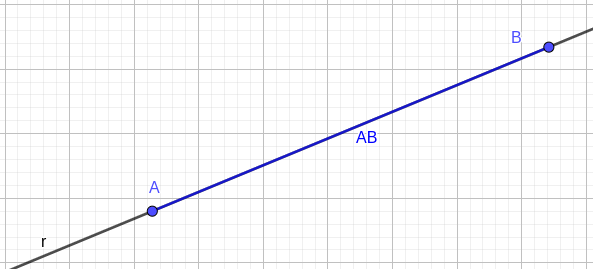
\includegraphics[width=0.7\textwidth]{./cap_vetor/dados/fig_segmento/fig_segmento}
  \caption{Esboço de um segmento $AB$.}
  \label{fig:segmento}
\end{figure}

Associado a um segmento $AB$, temos seu {\bf comprimento}\index{comprimento} (ou tamanho), o qual é definido como sendo a {\bf distância}\index{distância} entre os pontos $A$ e $B$. A distância entre os ponto $A$ e $B$ é denotada por $|AB|$ ou $|BA|$.

A {\bf direção} de um segmento $AB$ é a direção da reta que fica determinada pelos pontos $A$ e $B$.

\begin{ex}\label{ex:segmento}
  Consideremos os segmentos esboçados na Figura \ref{fig:ex_segmento}. Os segmentos $AB$ e $CD$ têm as mesmas direções, mas comprimentos diferentes. Já, o segmento $EF$ tem direção diferente dos segmentos $AB$ e $CD$.
  
  \begin{figure}[h!]
    \centering
    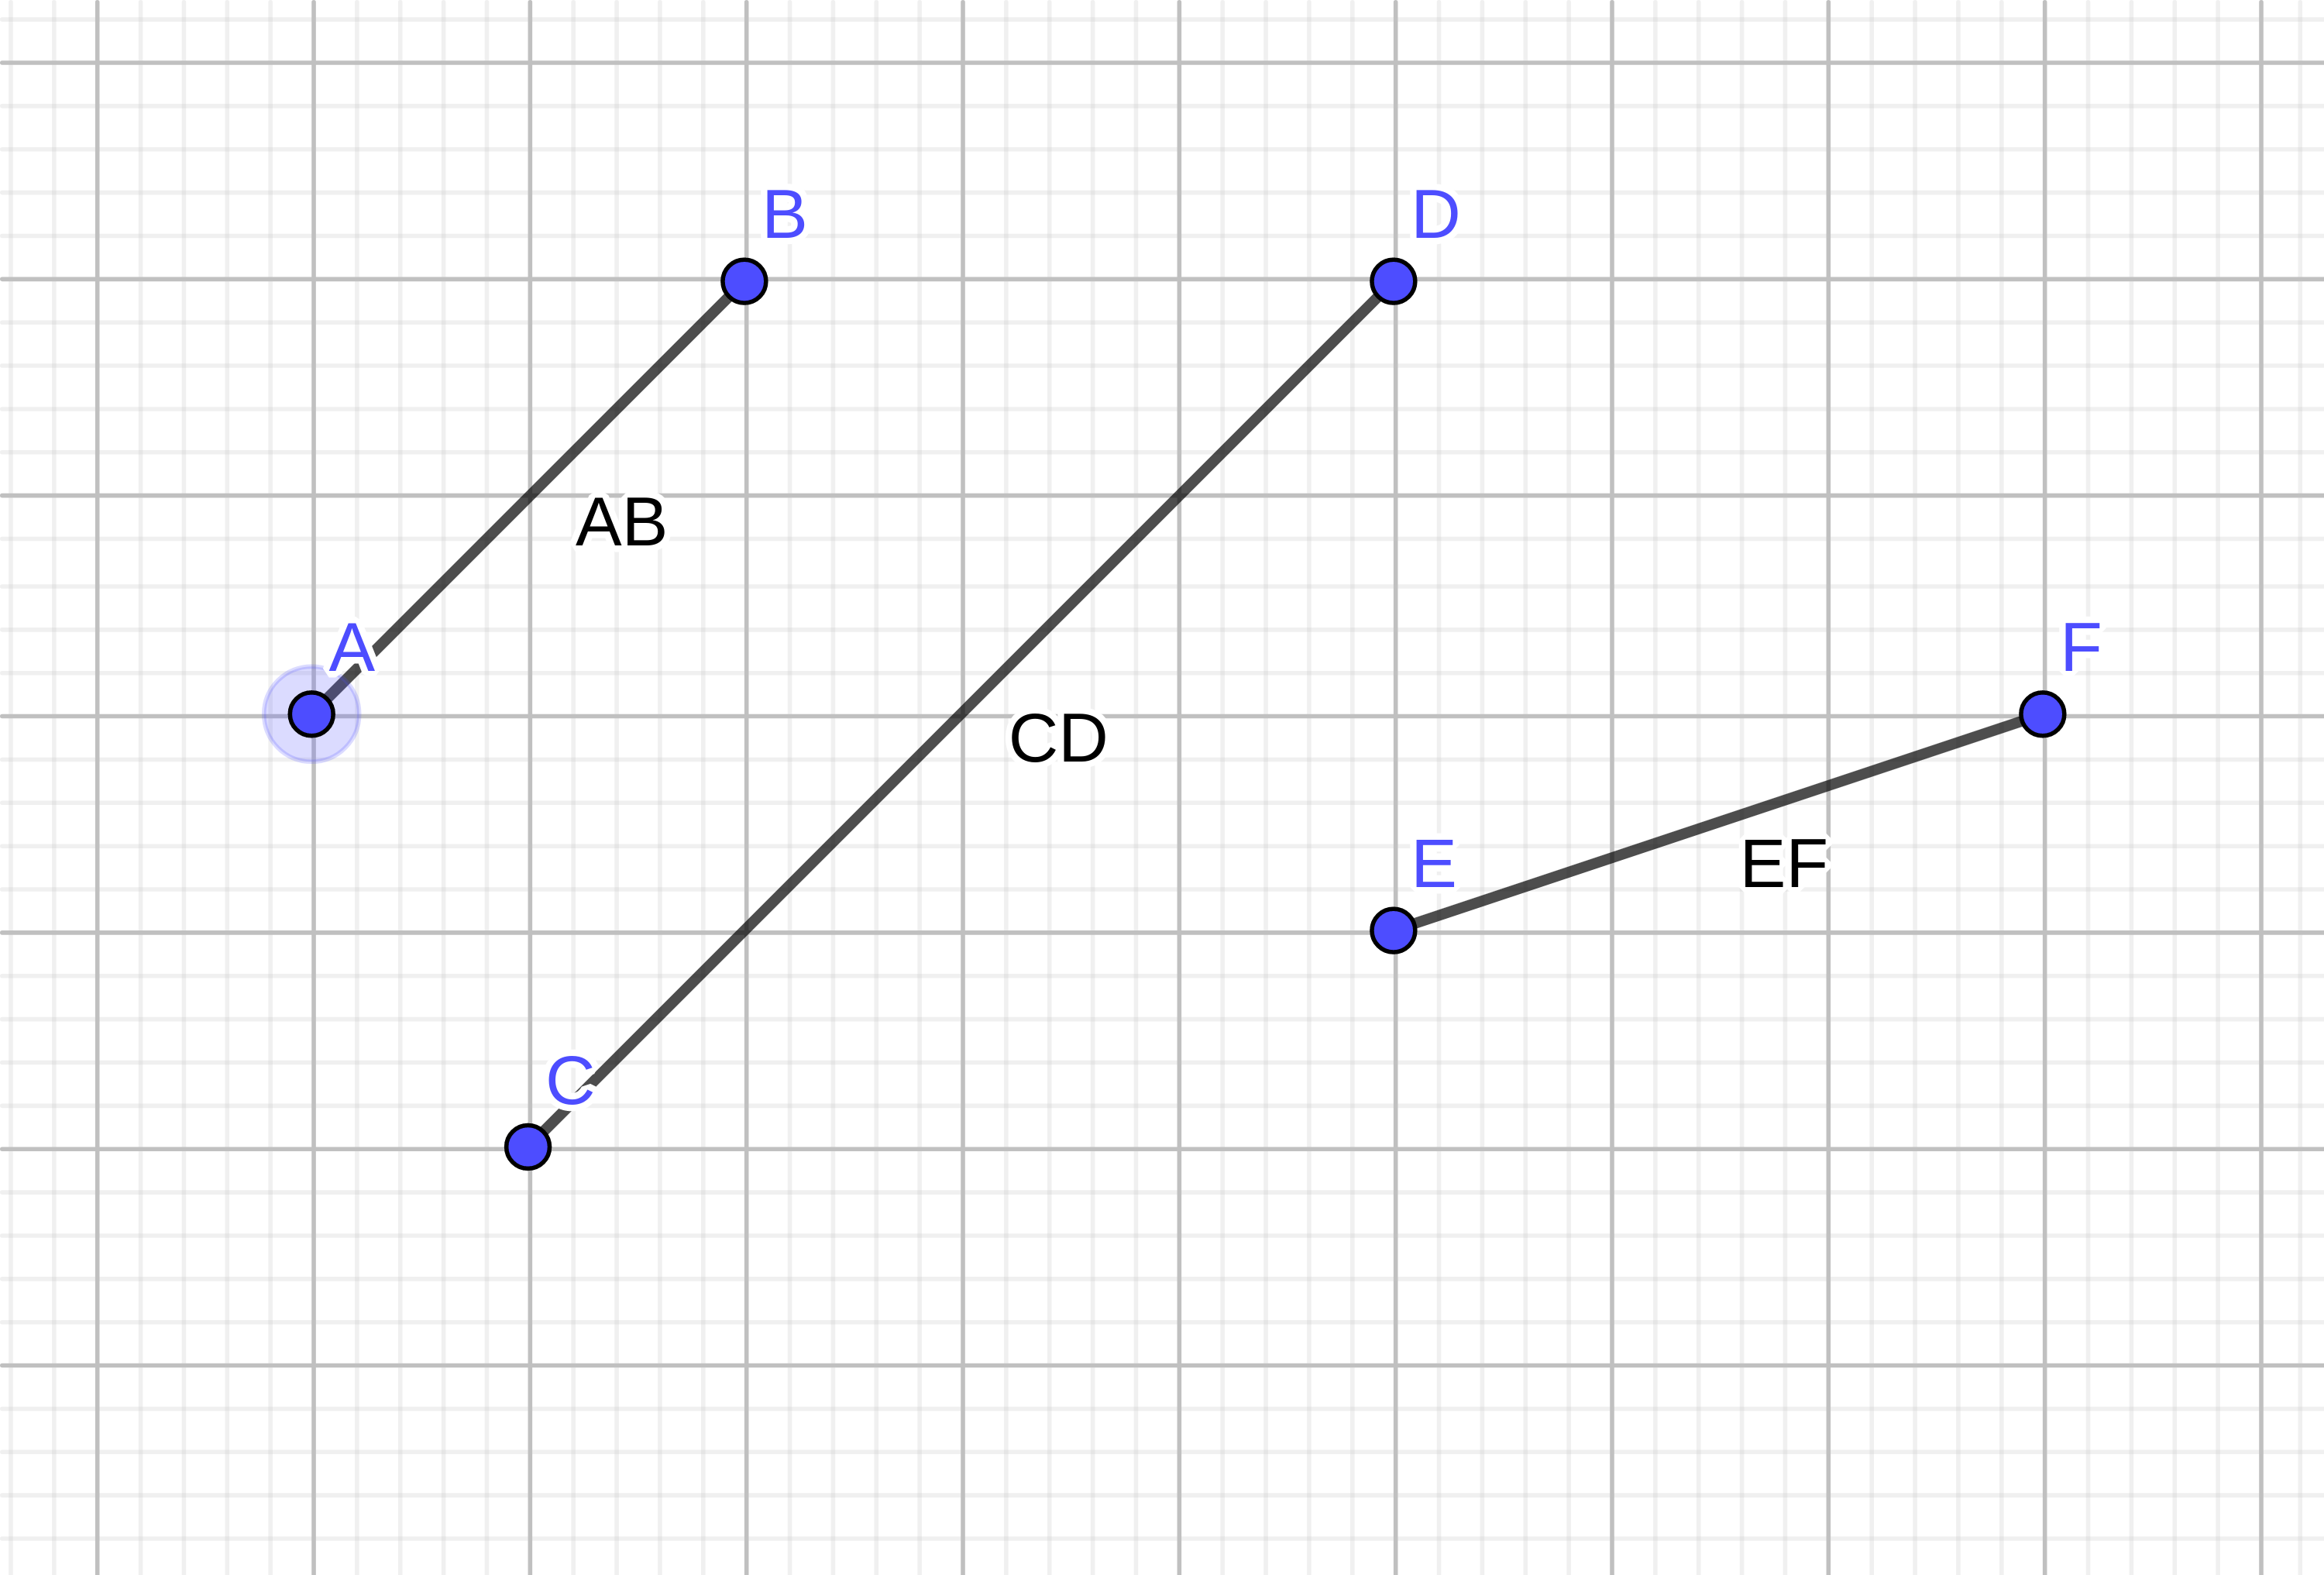
\includegraphics[width=0.7\textwidth]{./cap_vetor/dados/fig_ex_segmento/fig_ex_segmento}
  \caption{Esboço referente ao Exemplo \ref{ex:segmento}.}
  \label{fig:ex_segmento}
\end{figure}
\end{ex}

Se $A$ e $B$ são o mesmo ponto, então chamamos $AB$ de {\bf segmento nulo}\index{segmento nulo} e temos $|AB| = 0$. Um segmento nulo não tem direção.

\begin{figure}[h!]
  \centering
  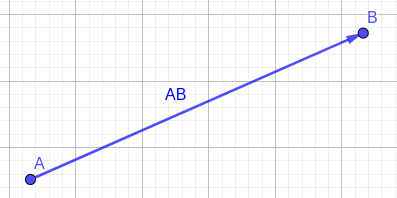
\includegraphics[width=0.7\textwidth]{./cap_vetor/dados/fig_seg_orientado/fig_seg_orientado}
  \caption{Esboço de um segmento orientado $AB$.}
  \label{fig:seg_orientado}
\end{figure}


Observemos que um dado segmento $AB$ é igual ao segmento $BA$. Agora, podemos associar a noção de {\bf sentido} a um segmento, escolhendo um dos pontos como sua {\bf origem}\index{origem} e o outro como sua {\bf extremidade}\index{extremidade}. Ao fazermos isso, definimos um {\bf segmento orientado}\index{segmento orientado}. Mais precisamente, um segmento orientado $AB$ é o segmento definido pelos pontos $A$ e $B$, sendo $A$ a origem e $B$ a extremidade. Veja a Figura \ref{fig:seg_orientado}.

Dizemos que dois dados segmentos orientados não nulos $AB$ e $CD$ têm a {\bf mesma direção} quando as retas $AB$ e $CD$ forem paralelas ou coincidentes.

\begin{ex}\label{ex:segorien_direcao}
  Consideremos os segmentos orientados esboçados na Figura \ref{fig:ex_segorien_direcao}. Observemos que os segmentos orientados $AB$ e $CD$ têm a mesma direção. Já o segmento orientado $EF$ tem direção diferente dos segmentos $AB$ e $CD$.
  
  \begin{figure}[h!]
    \centering
    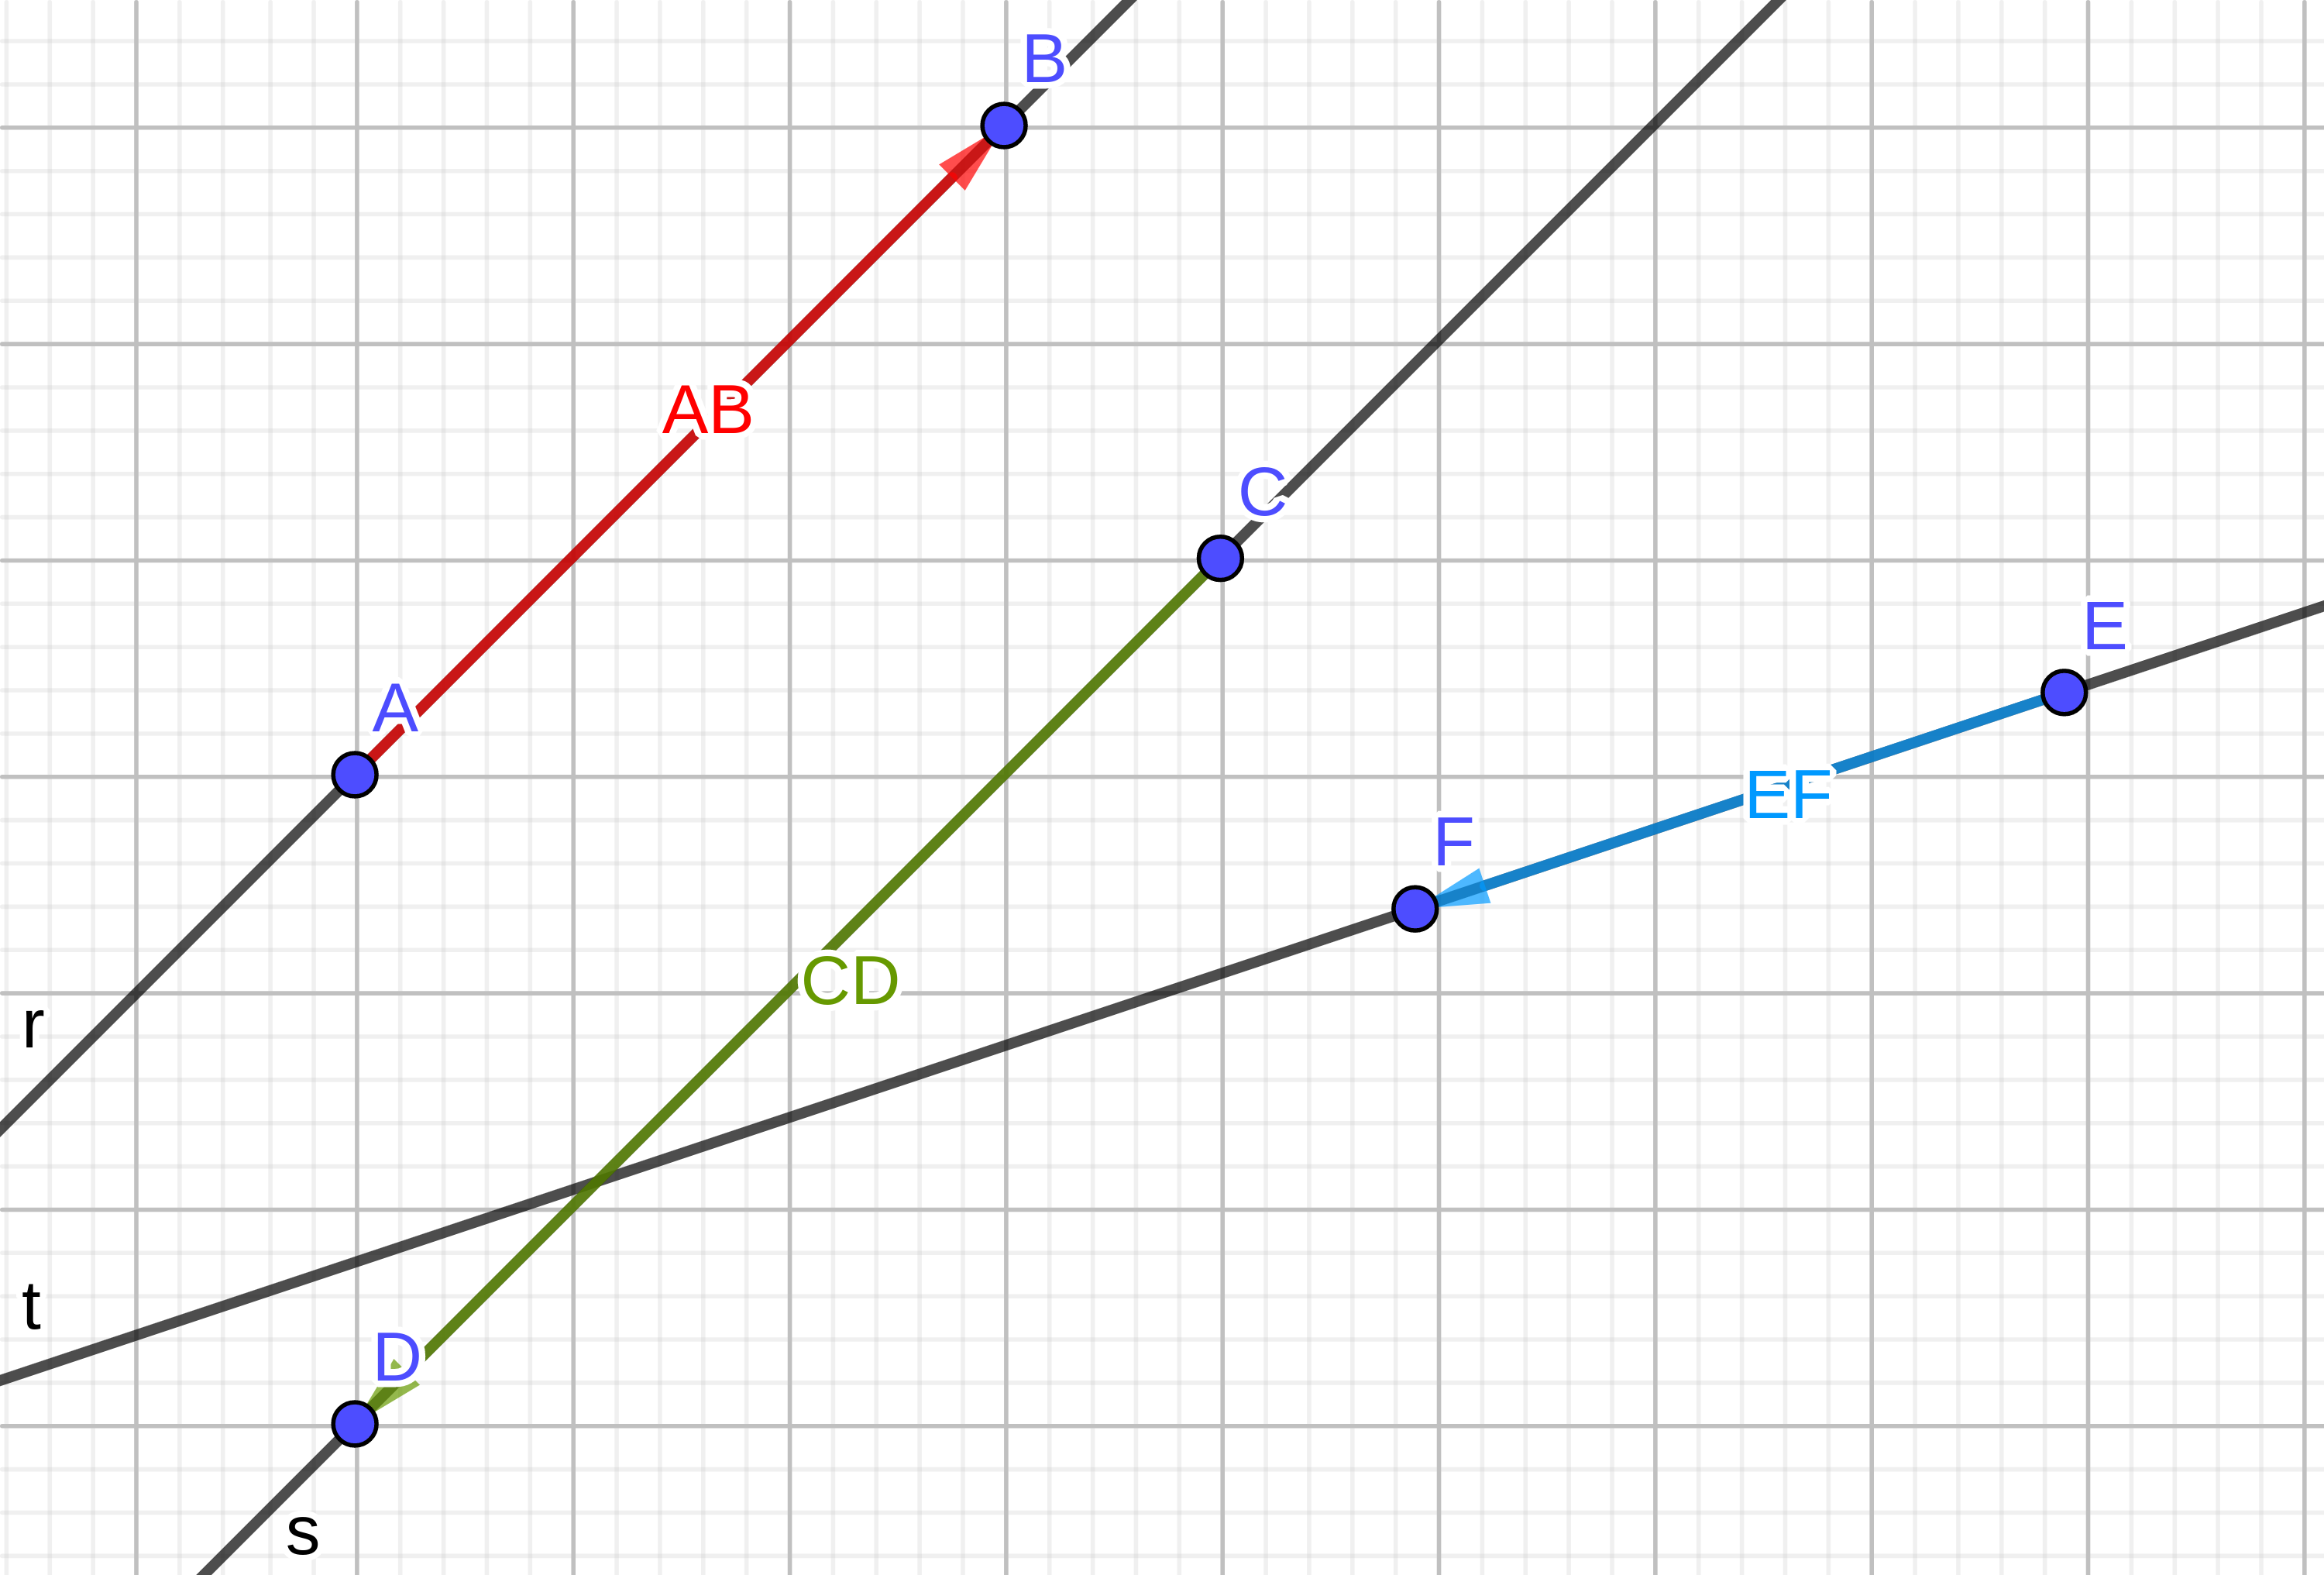
\includegraphics[width=0.7\textwidth]{./cap_vetor/dados/fig_ex_segorien_direcao/fig_ex_segorien_direcao}
  \caption{Esboço referente ao Exemplo \ref{ex:segorien_direcao}.}
  \label{fig:ex_segorien_direcao}
\end{figure}  
\end{ex}

Sejam dados dois segmentos orientados $AB$ e $CD$ de mesma direção, cujas retas $AB$ e $CD$ não sejam coincidentes. Então, as retas $AB$ e $CD$ determinam um único plano e a reta $AC$ determina dois semiplanos (veja a Figura \ref{fig:segorien_sentido}). Assim sendo, dizemos que os segmentos $AB$ e $CD$ têm {\bf mesmo sentido}\index{mesmo sentido} quando os pontos $B$ e $D$ estão ambos sobre o mesmo semiplano.

\begin{figure}[h!]
  \centering
  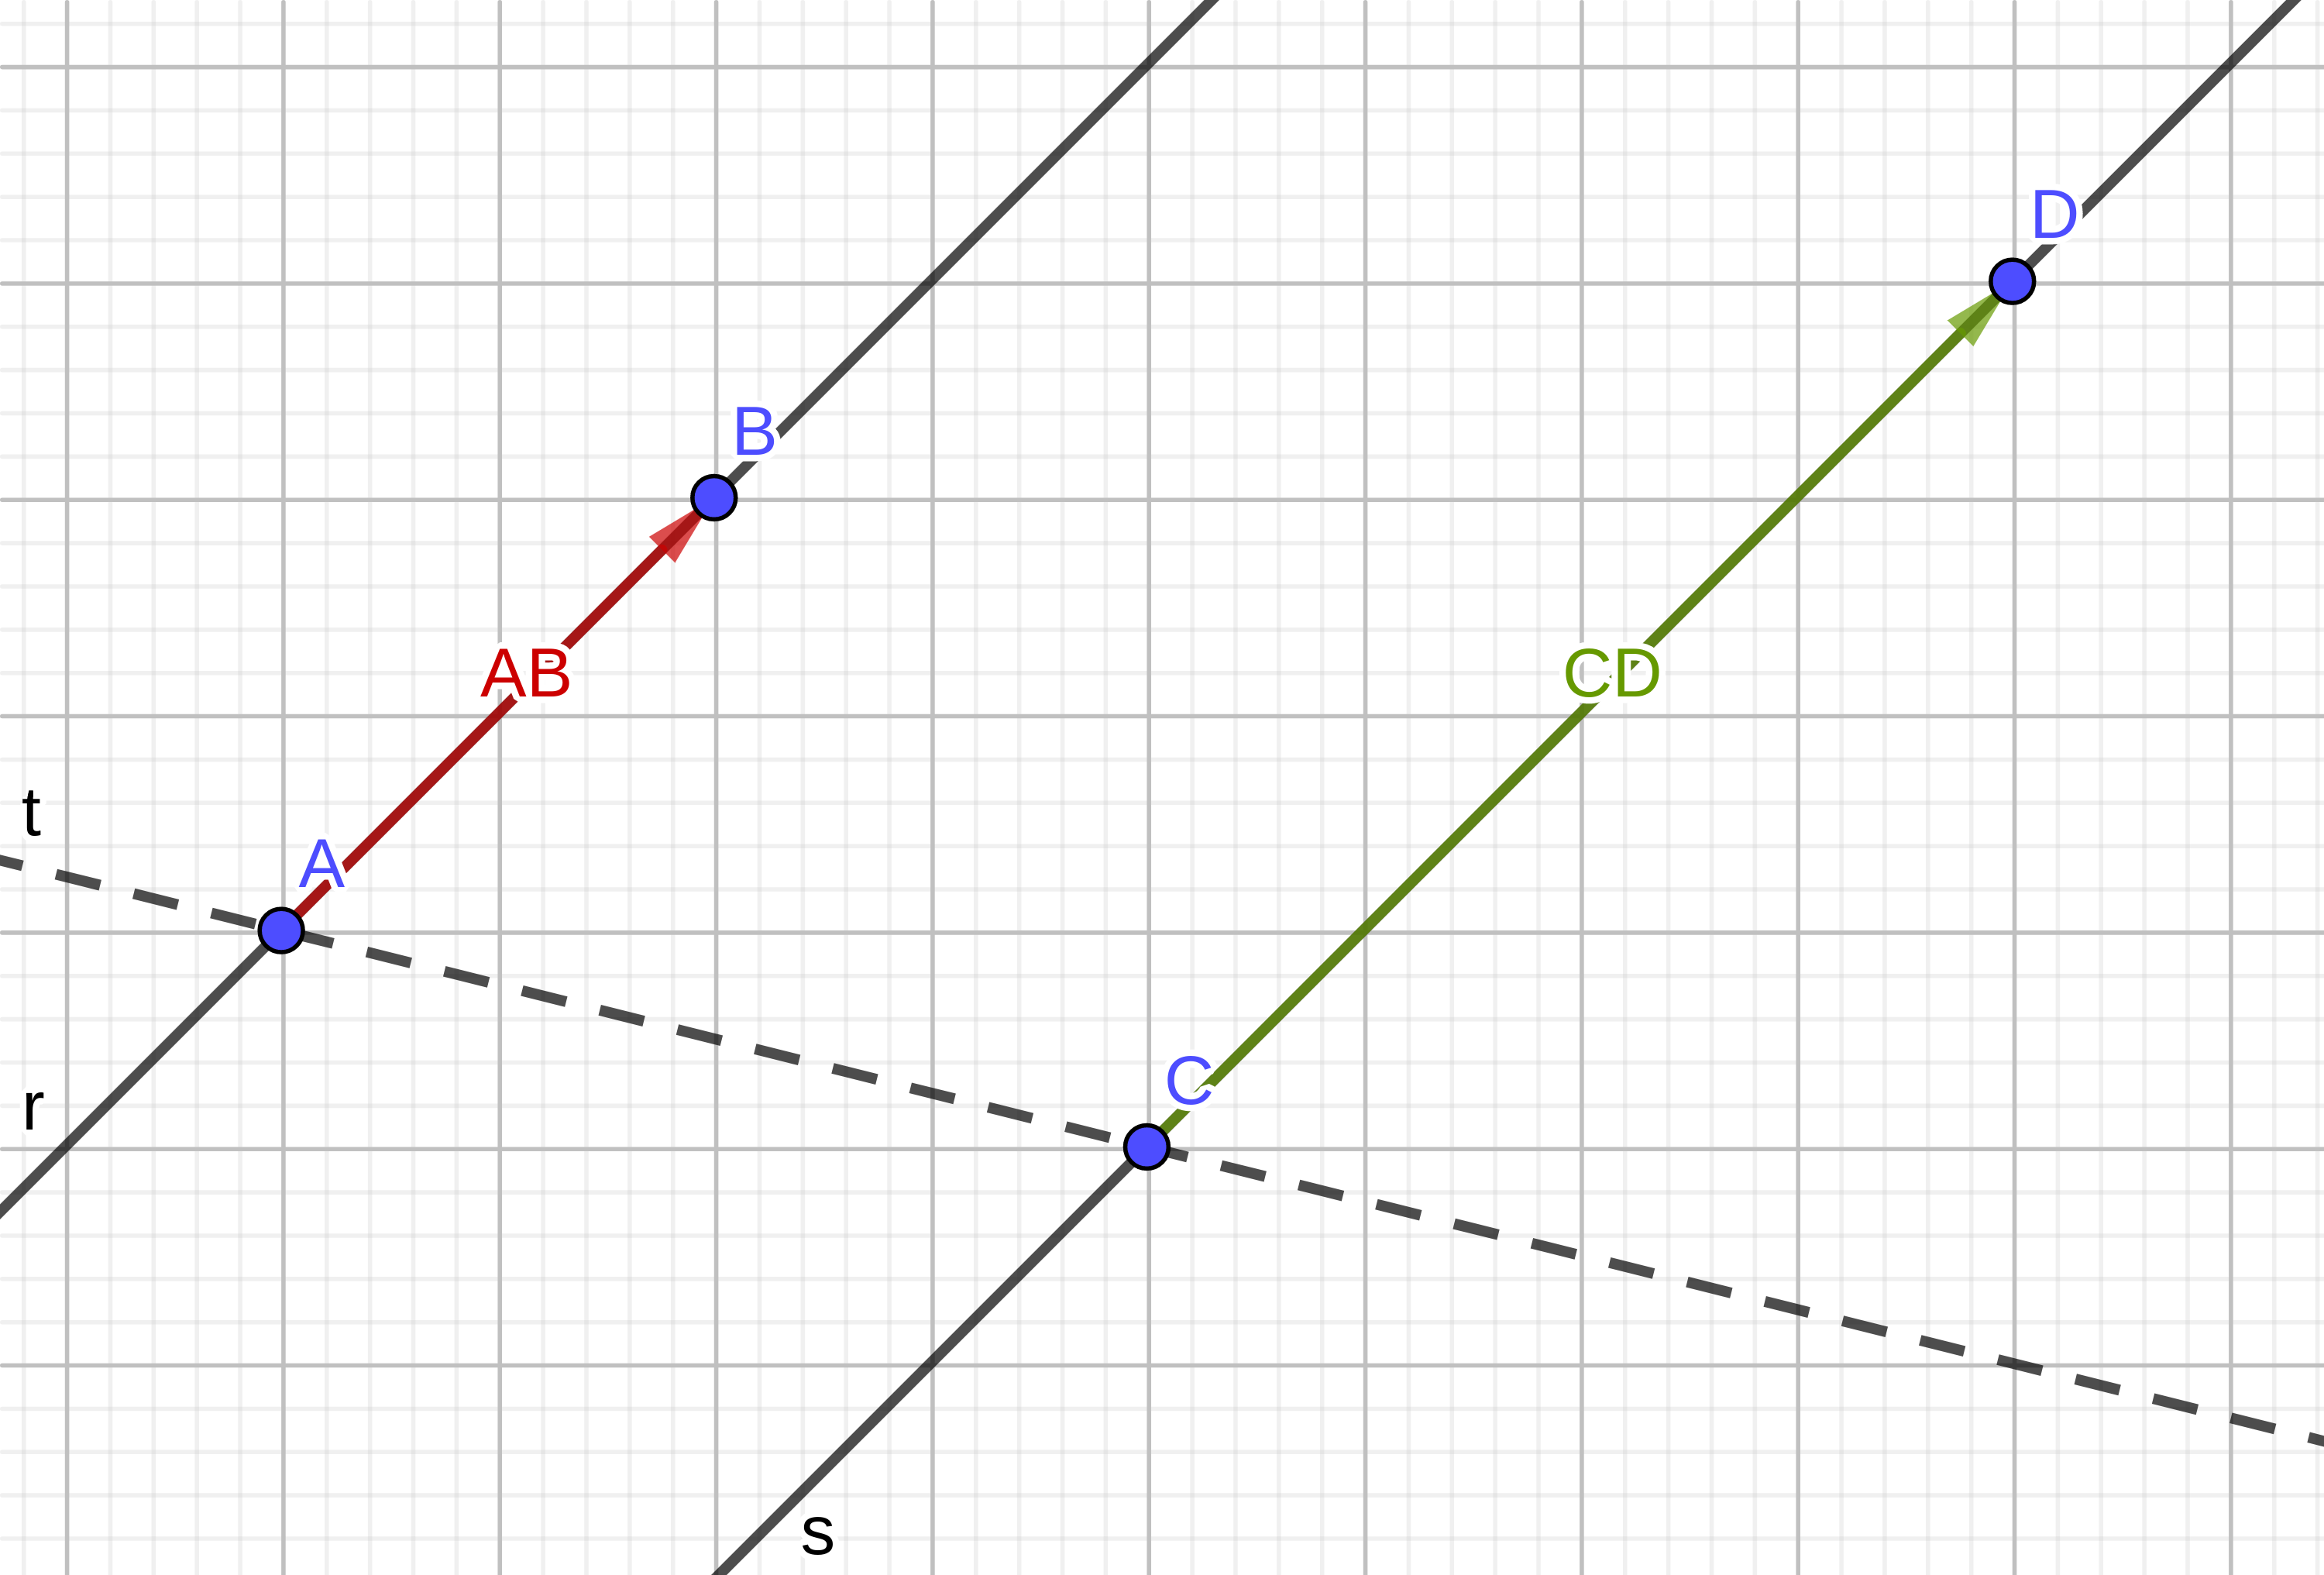
\includegraphics[width=0.7\textwidth]{./cap_vetor/dados/fig_segorien_sentido/fig_segorien_sentido}
  \caption{Esboço de dois segmentos orientados $AB$ e $CD$ de mesmo sentido.}
  \label{fig:segorien_sentido}
\end{figure}

Para analisar o sentido de dois segmentos orientados e colineares, escolhemos um deles e construímos um segmento orientado de mesmo sentido a este, mas não colinear. Então, analisamos o sentido dos segmentos orientados originais com respeito ao introduzido.

Dois segmentos orientados não nulos são {\bf equipolentes}\index{equipolentes} quando eles têm o mesmo comprimento, mesma direção e mesmo sentido. Veja o exemplo dado na Figura \ref{fig:segequipolentes}. Segmentos nulos também são considerados equipolentes entre si. Quando $AB$ é equipolente a $CD$, escrevemos $AB \sim CD$.

\begin{figure}[h!]
  \centering
  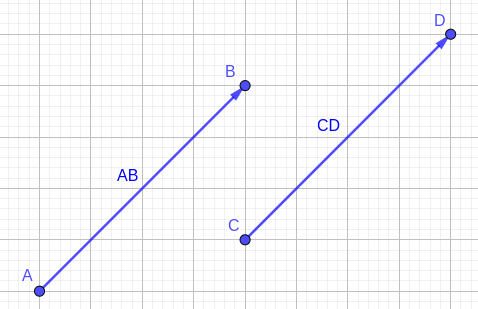
\includegraphics[width=0.7\textwidth]{./cap_vetor/dados/fig_segequipolentes/fig_segequipolentes}
  \caption{Esboço de dois segmentos orientados $AB$ e $CD$ equipolentes.}
  \label{fig:segequipolentes}
\end{figure}

A relação de equipolência é uma \emph{relação de equivalência}. De fato, temos:
\begin{itemize}
\item \emph{relação reflexiva}: $AB \sim AB$;
\item \emph{relação simétrica}: $AB \sim CD \Rightarrow CD \sim AB$;
\item \emph{relação transitiva}: $AB \sim CD ~ \text{e} ~ CD \sim EF \Rightarrow AB \sim CD$.
\end{itemize}

Com isso, dado um segmento $AB$, definimos a \emph{classe de equipolência} de $AB$ como o conjunto de todos os segmentos equipolentes a $AB$. O segmento $AB$ é um \emph{representante} desta classe.

\subsection*{Exercícios resolvidos}

\begin{exeresol}
  Mostre que dois segmentos orientados $AB$ e $CD$ são equipolentes se, e somente se, os pontos médios de $AD$ e $BC$ são coincidentes.
\end{exeresol}
\begin{resol}
  Começamos mostrando a implicação. Por hipótese, temos que $AB$ e $CD$ são equipolentes. A tese é clara no caso de $AB$ e $CD$ serem coincidentes. Vejamos, então, o caso em que $AB$ e $CD$ não são coincidentes. Desta forma, $ABCD$ determina um paralelogramo de diagonais $AD$ e $BC$. Como as diagonais de um paralelogramo se interceptam em seus pontos médios, temos demonstrado a implicação.

  Agora, mostramos a recíproca. Por hipótese, temos que os pontos médios de $AD$ e $BC$ são coincidentes. Novamente, se $AD$ e $BD$ são coincidentes a conclusão é direta. Consideremos o caso em que $AD$ e $BD$ não são coincidentes. Daí, segue que $AB$ e $CD$ têm o mesmo tamanho e mesma direção. Seja $M$ o ponto médio de $AD$ e $BC$ e $\pi$ o plano determinado pelos segmentos $AB$ e $CD$. Notando que $M$, $B$ e $D$ estão no mesmo semiplano de $\pi$ determinado pela reta $AC$, concluímos que $AB$ e $CD$ são equipolentes.
\end{resol}

\begin{exeresol}
  Mostre que $AB\sim CD$, então $BA\sim DC$.
\end{exeresol}
\begin{resol}
  $AB$ e $BA$ têm o mesmo tamanho e direção. $CD$ e $DC$ têm o mesmo tamanho e direção. Como $AB\sim CD$, temos que $BA$ e $DC$ têm o mesmo tamanho e direção. Por fim, observa-se que $BA$ e $DC$ têm ambos o mesmo sentido oposto de $AB$ e $DC$. 
\end{resol}

\subsection*{Exercícios}

\begin{exer}
  Faça o esboço de dois segmentos $AB$ e $CD$ com $|AB|\neq |CD|$ e cujas retas determinadas por eles sejam coincidentes.
\end{exer}

\begin{exer}
  Faça o esboço de dois segmentos orientados $AB\not\sim CD$ e de mesmo sentido.
\end{exer}

\begin{exer}
  Faça o esboço de dois segmentos orientados colineares, de tamanhos iguais e sentidos opostos.
\end{exer}

\begin{exer}
  Diga se é verdadeira ou falsa a seguinte afirmação: é quadrado todo trapézio retângulo $ABCD$ com segmentos orientados $AD$ e $BC$ equipolentes. Justifique sua afirmação. 
\end{exer}
\begin{resp}
  Verdadeira.
\end{resp}

\begin{exer}
  Mostre que $AB\sim CD$, então $AC\sim BD$.
\end{exer}
\begin{resp}
  Dica: $ABCD$ determina um paralelogramo.
\end{resp}

\begin{exer}
  Mostre que se $AC\sim CB$, então $C$ é ponto médio do segmento $AB$.
\end{exer}

\section{Vetores}\label{cap_vetor_sec_vetor}

Dado um segmento orientado $AB$, chama-se {\bf vetor} $AB$ e denota-se $\overrightarrow{AB}$, qualquer segmento orientado equipolente a $AB$. Em outras palavras, o vetor $\overrightarrow{AB}$ é a classe de equipolência que tem o segmento orientado $AB$ como um representante. A Figura \ref{fig:vetor} mostra duas representações de um dado vetor $\overrightarrow{AB}$.

\begin{figure}[h!]
  \centering
  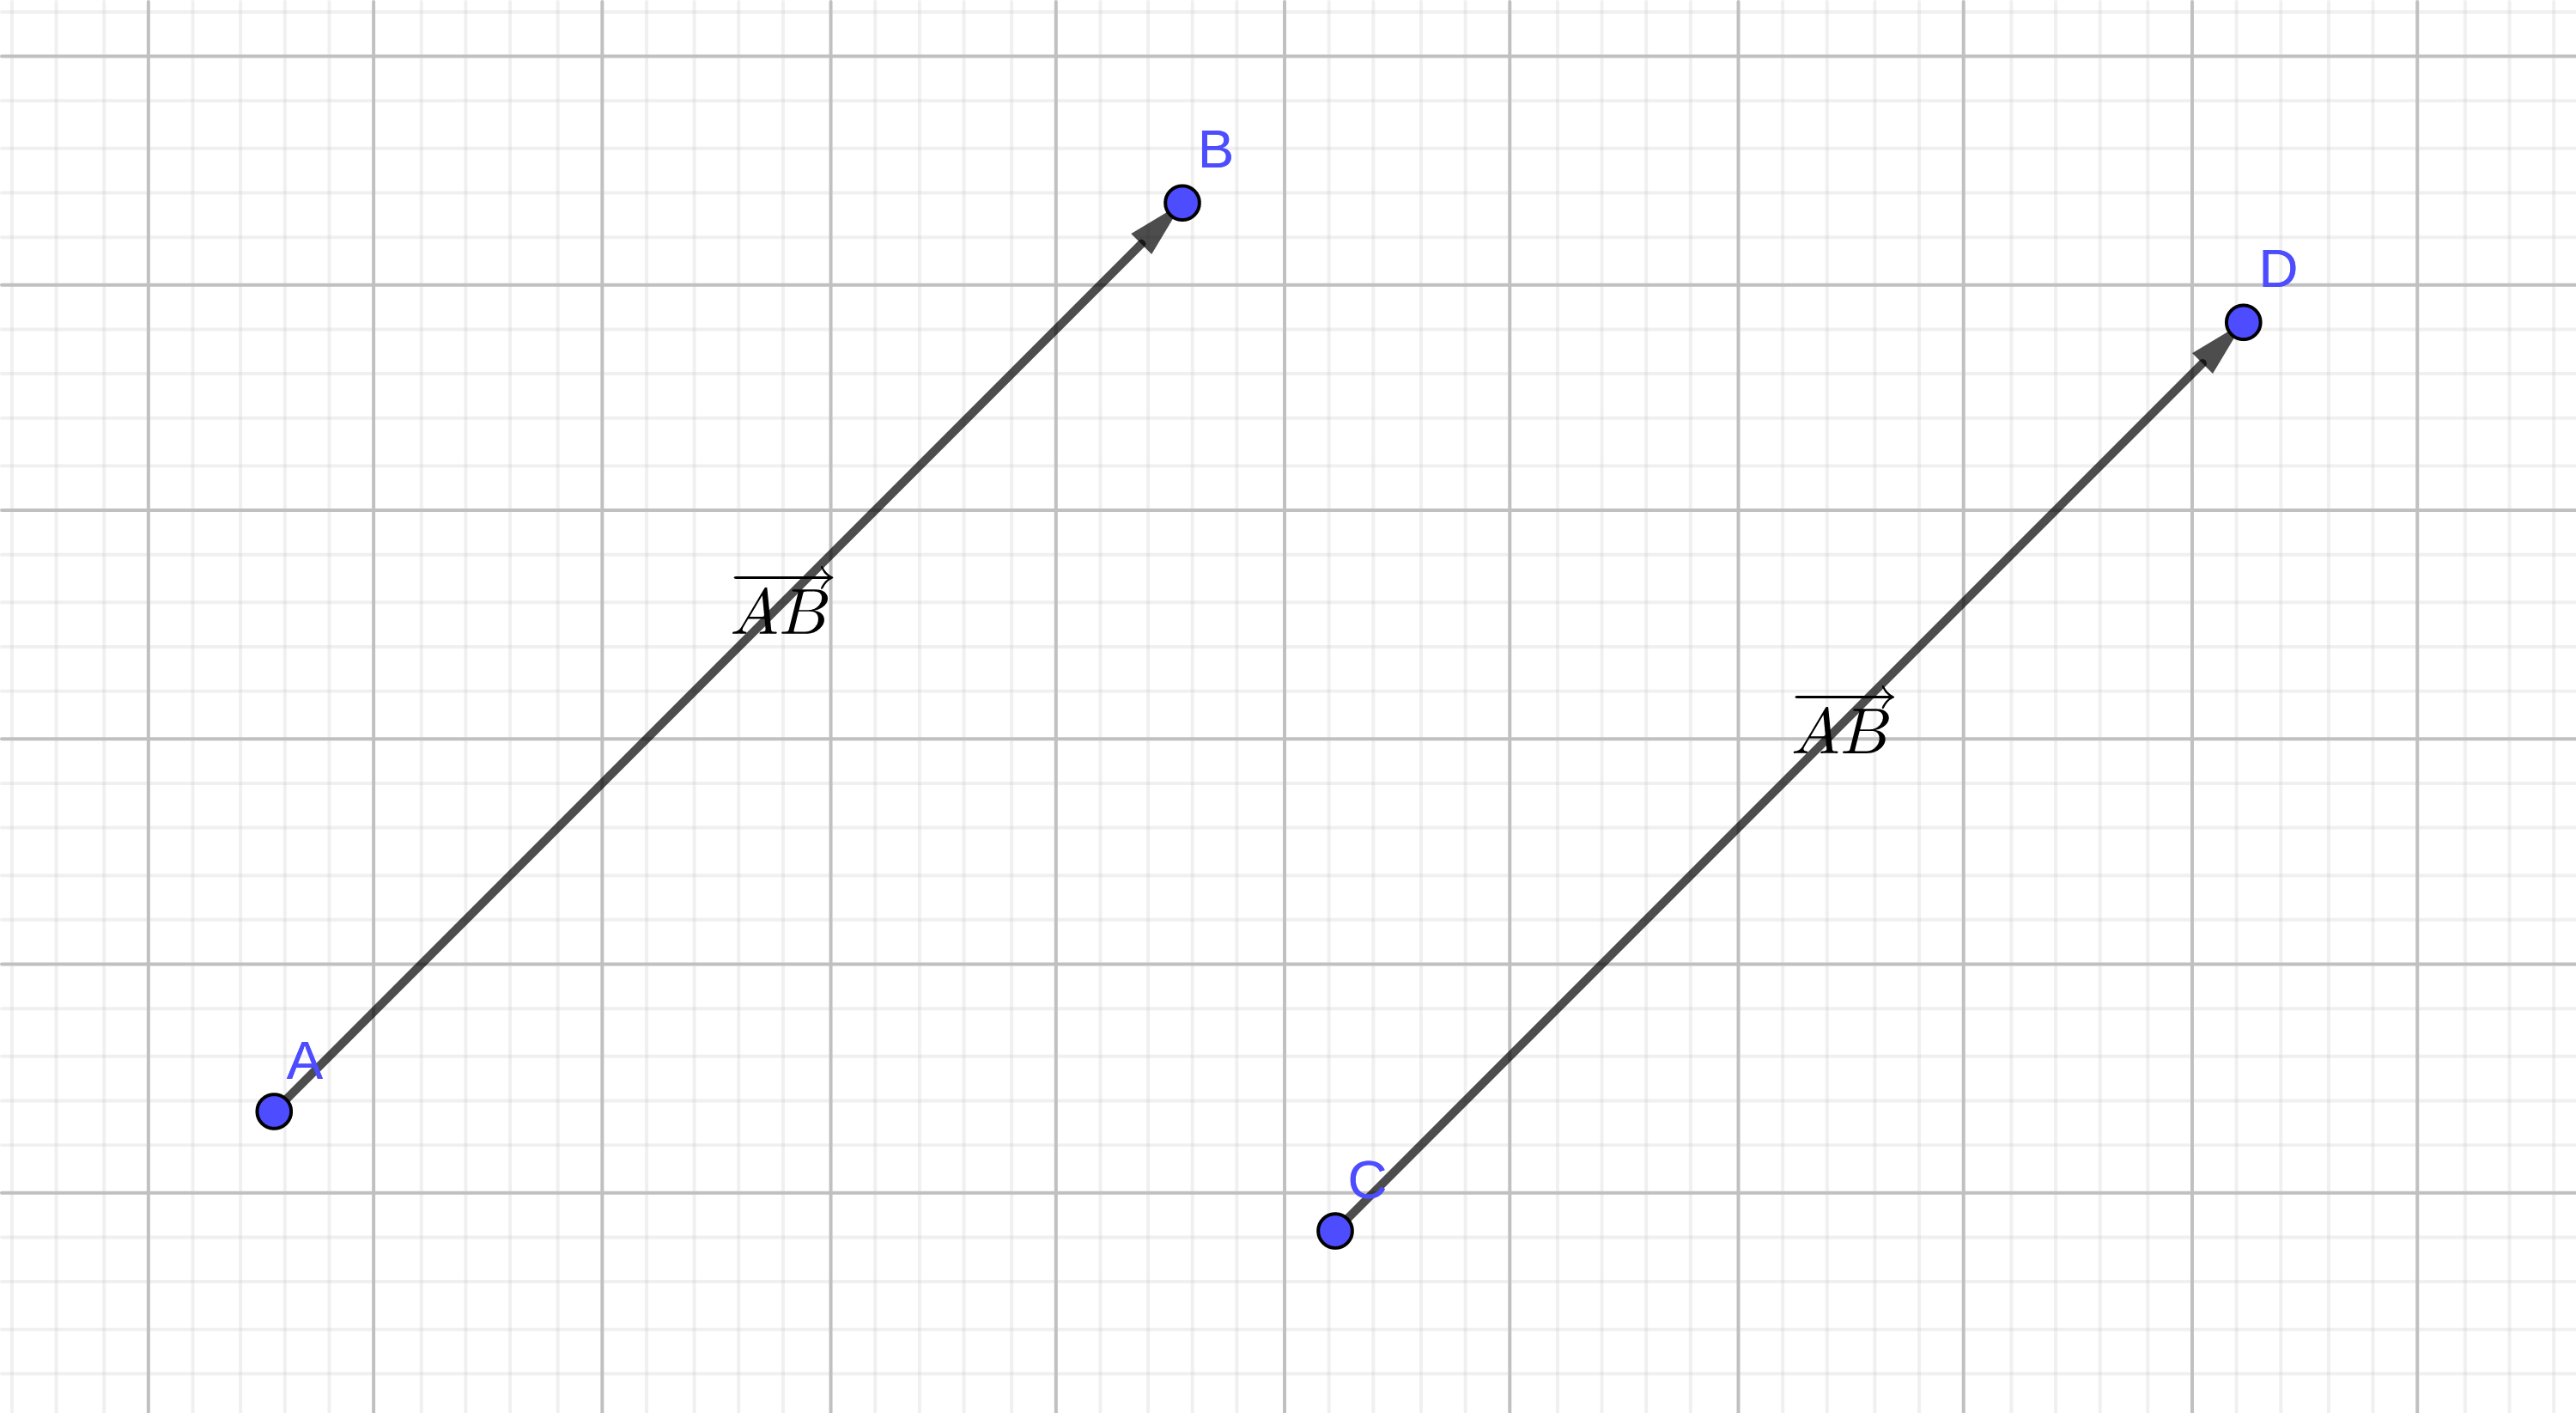
\includegraphics[width=0.7\textwidth]{./cap_vetor/dados/fig_vetor/fig_vetor}
  \caption{Esboço de duas representações de um mesmo vetor.}
  \label{fig:vetor}
\end{figure}

Observemos que na Figura \ref{fig:vetorrel}(direita) os vetores foram denotados por $\vec{a}$, $\vec{b}$ e $\vec{c}$, sem alusão aos pontos que definem suas representações como segmentos orientados. Isto é costumeiro, devido a definição de vetor.

O \emph{vetor nulo} é aquele que tem como seu representante um segmento orientado nulo. É denotado por $\vec{0}$.

O {\bf módulo}\index{módulo} (ou {\bf norma}\index{norma}) de um vetor $\vec{v}$ é denotado(a) por $|\vec{v}|$ e é definido como o valor do comprimento de qualquer uma de suas representações. Mais precisamente, se $\overrightarrow{AB}$ é uma representação de $\vec{v}$, então $|\vec{v}| := |\overrightarrow{AB}|$.

\begin{obs}
  $|\vec{v}| = 0$ se, e somente se, $\vec{v} = \vec{0}$.

  Seja $\vec{v} = \overrightarrow{AB}$. Lembrando que $|\overrightarrow{AB}| = |AB|$, i.e. a distância entre os pontos $A$ e $B$, segue que se $\vec{v} = \vec{0}$, então $A$ e $B$ são dois pontos sobrepostos e, portanto, $|\vec{v}| = |AB| = 0$. Reciprocamente, se $|AB| = 0$, então $A$ e $B$ são sobrepostos e $\overrightarrow{AB} = \vec{0}$.
\end{obs}

Dois {\bf vetores} são ditos {\bf paralelos} \index{vetores!paralelos} quando qualquer de suas representações têm a mesma direção. De forma análoga, definem-se {\bf vetores coplanares}\index{vetores!coplanares}, {\bf vetores não coplanares}\index{vetores!não coplanares}, {\bf vetores ortogonais}\index{vetores!ortogonais}, além de conceitos como {\bf ângulo entre dois vetores}\index{ângulo!entre vetores}, etc. Veja a Figura \ref{fig:vetorrel}.

\begin{figure}[h!]
  \centering
  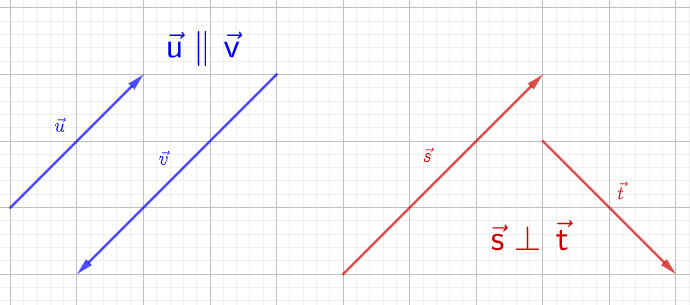
\includegraphics[width=0.5\textwidth]{./cap_vetor/dados/fig_vetorrel/fig_vetorrel}~
  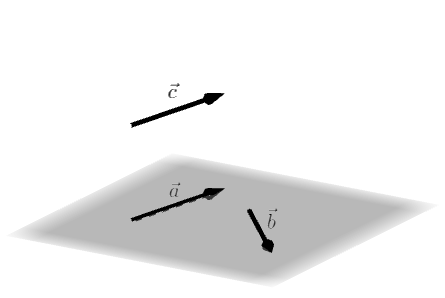
\includegraphics[width=0.5\textwidth]{./cap_vetor/dados/fig_vcolineares/fig_vcolineares}
  \caption{Esquerda: esboços de vetores paralelos e de vetores ortogonais. Direita: esboços de vetores coplanares.}
  \label{fig:vetorrel}
\end{figure}

\subsection{Adição de vetores}

Sejam dados dois vetores $\vec{u}$ e $\vec{v}$. Sejam, ainda, uma representação $\overrightarrow{AB}$ qualquer de $\vec{u}$ e uma representação $\overrightarrow{BC}$ do vetor $\vec{v}$. Então, define-se o vetor soma $\vec{u}+\vec{v}$ como o vetor representado por $\overrightarrow{AC}$. Veja a Figura \ref{fig:vadicao}.

\begin{figure}[H]
  \centering
  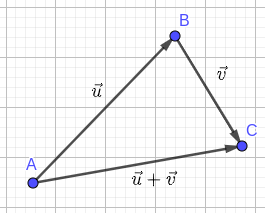
\includegraphics[width=0.7\textwidth]{./cap_vetor/dados/fig_vadicao/fig_vadicao}
  \caption{Representação geométrica da adição de dois vetores.}
  \label{fig:vadicao}
\end{figure}

\begin{obs}
  Vejamos as seguintes propriedades:
  \begin{enumerate}[a)]
  \item Elemento neutro na adição:
    \begin{equation}
      \vec{u} + \vec{0} = \vec{u}
    \end{equation}
    
    De fato, seja $\vec{u} = \overrightarrow{AB}$. Observamos que podemos representar $\vec{0} = \overrightarrow{BB}$. Logo, temos $\vec{u} + \vec{0} = \overrightarrow{AB} + \overrightarrow{BB} = \overrightarrow{AB} = \vec{u}$.

  \item Associatividade na adição:
    \begin{equation}
      (\vec{u} + \vec{v}) + \vec{w} = \vec{u} + (\vec{v} + \vec{w}).
    \end{equation}

    De fato, sejam $\vec{u} = \overrightarrow{AB}$, $\vec{v} = \overrightarrow{BC}$ e $\vec{w} = \overrightarrow{CD}$. Então, segue
    \begin{align}
      \left(\vec{u} + \vec{v}\right)+\vec{w} &= \left(\overrightarrow{AB}+\overrightarrow{BC}\right)+\overrightarrow{CD} \\
                                             &= \overrightarrow{AC} + \overrightarrow{CD} \\
                                             &= \overrightarrow{AD},
    \end{align}
    bem como,
    \begin{align}
      \vec{u} + \left(\vec{v} + \vec{w}\right) &= \overrightarrow{AB}+\left(\overrightarrow{BC}+\overrightarrow{CD}\right) \\
                                             &= \overrightarrow{AB} + \overrightarrow{BD} \\
                                             &= \overrightarrow{AD}.
    \end{align}
  \item Comutatividade da adição:
    \begin{equation}
      \vec{u} + \vec{v} = \vec{v} + \vec{u}.
    \end{equation}

    Esta propriedade pode ser demonstrada usando a regra do paralelograma que veremos mais adiante. Veja, também, o Exercício Resolvido \ref{exeresol:vetor_comuta_adicao}.
  \end{enumerate}
\end{obs}

\subsection{Vetor oposto}

Um \pmb{vetor} $\vec{v}$ é dito ser \pmb{oposto} \index{vetor!oposto} a um dado vetor $\vec{u}$, quando quaisquer representações de $\vec{u}$ e $\vec{v}$ são segmentos orientados de mesmo comprimento e mesma direção, mas com sentidos opostos. Neste caso, denota-se por $-\vec{u}$ o vetor oposto a $\vec{u}$. Veja a Figura \ref{fig:voposto}.

\begin{figure}[H]
  \centering
  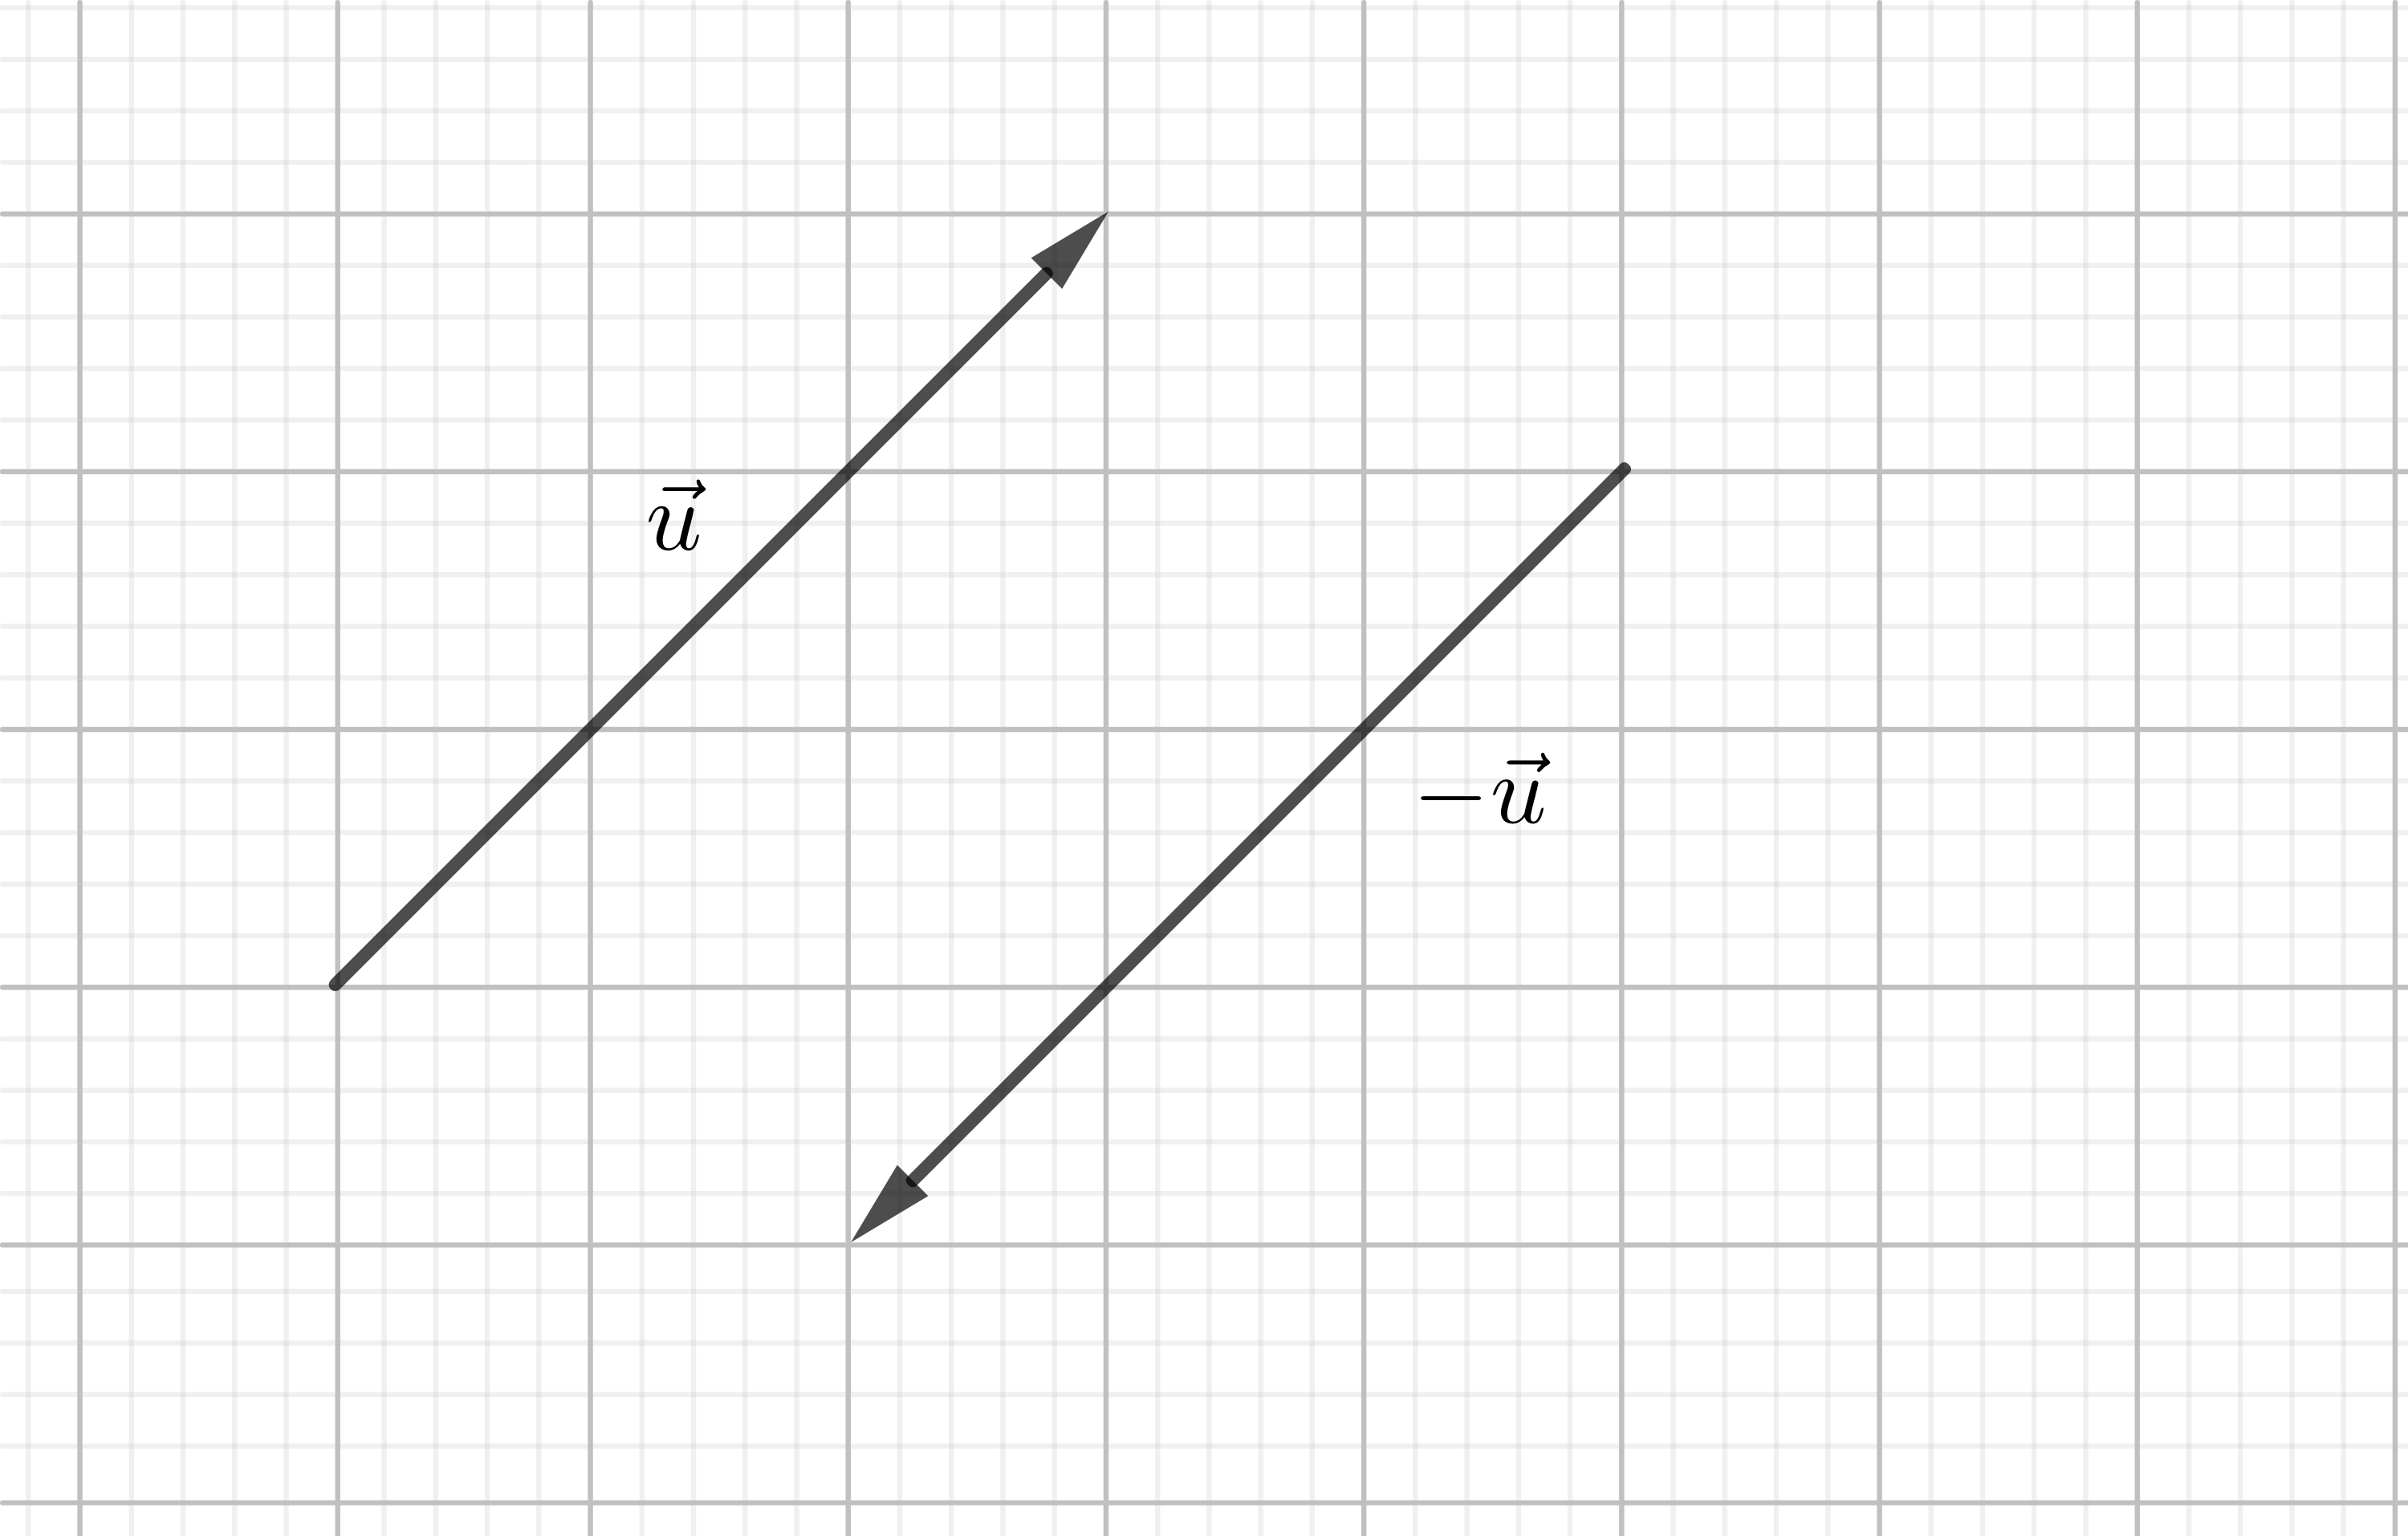
\includegraphics[width=0.7\textwidth]{./cap_vetor/dados/fig_voposto/fig_voposto}
  \caption{Representação geométrica de vetores opostos.}
  \label{fig:voposto}
\end{figure}

\begin{obs}
  $|\vec{v}| = |-\vec{v}|$.

  De fato, seja $\vec{v} = \overrightarrow{AB}$. Então, $|\vec{v}| = |AB| = |BA| = |-\vec{v}|$.
\end{obs}

\begin{obs}(Existência do oposto)
  \begin{equation}
    \vec{u} + \left(-\vec{u}\right) = \vec{0}.
  \end{equation}

  De fato, seja $\vec{u} = \overrightarrow{AB}$. Então, $-\vec{u} = -\overrightarrow{AB} = \overrightarrow{BA}$. Segue que
  \begin{align}
    \vec{u} + \left(-\vec{u}\right) &= \overrightarrow{AB} + \left(-\overrightarrow{AB}\right) \\
                                    &= \overrightarrow{AB} + \overrightarrow{BA} \\
                                    &= \overrightarrow{AA} \\
                                    &= \vec{0}.
  \end{align}
\end{obs}

\subsection{Subtração de vetores}

Sejam dados dois vetores $\vec{u}$ e $\vec{v}$. A subtração de $\vec{u}$ com $\vec{v}$ é denotada por $\vec{u}-\vec{v}$ e é definida pela adição de $\vec{u}$ com $-\vec{v}$, i.e. $\vec{u}-\vec{v}=\vec{u}+(-\vec{v})$. Veja a Figura \ref{fig:vsubtracao}.

\begin{figure}[H]
  \centering
  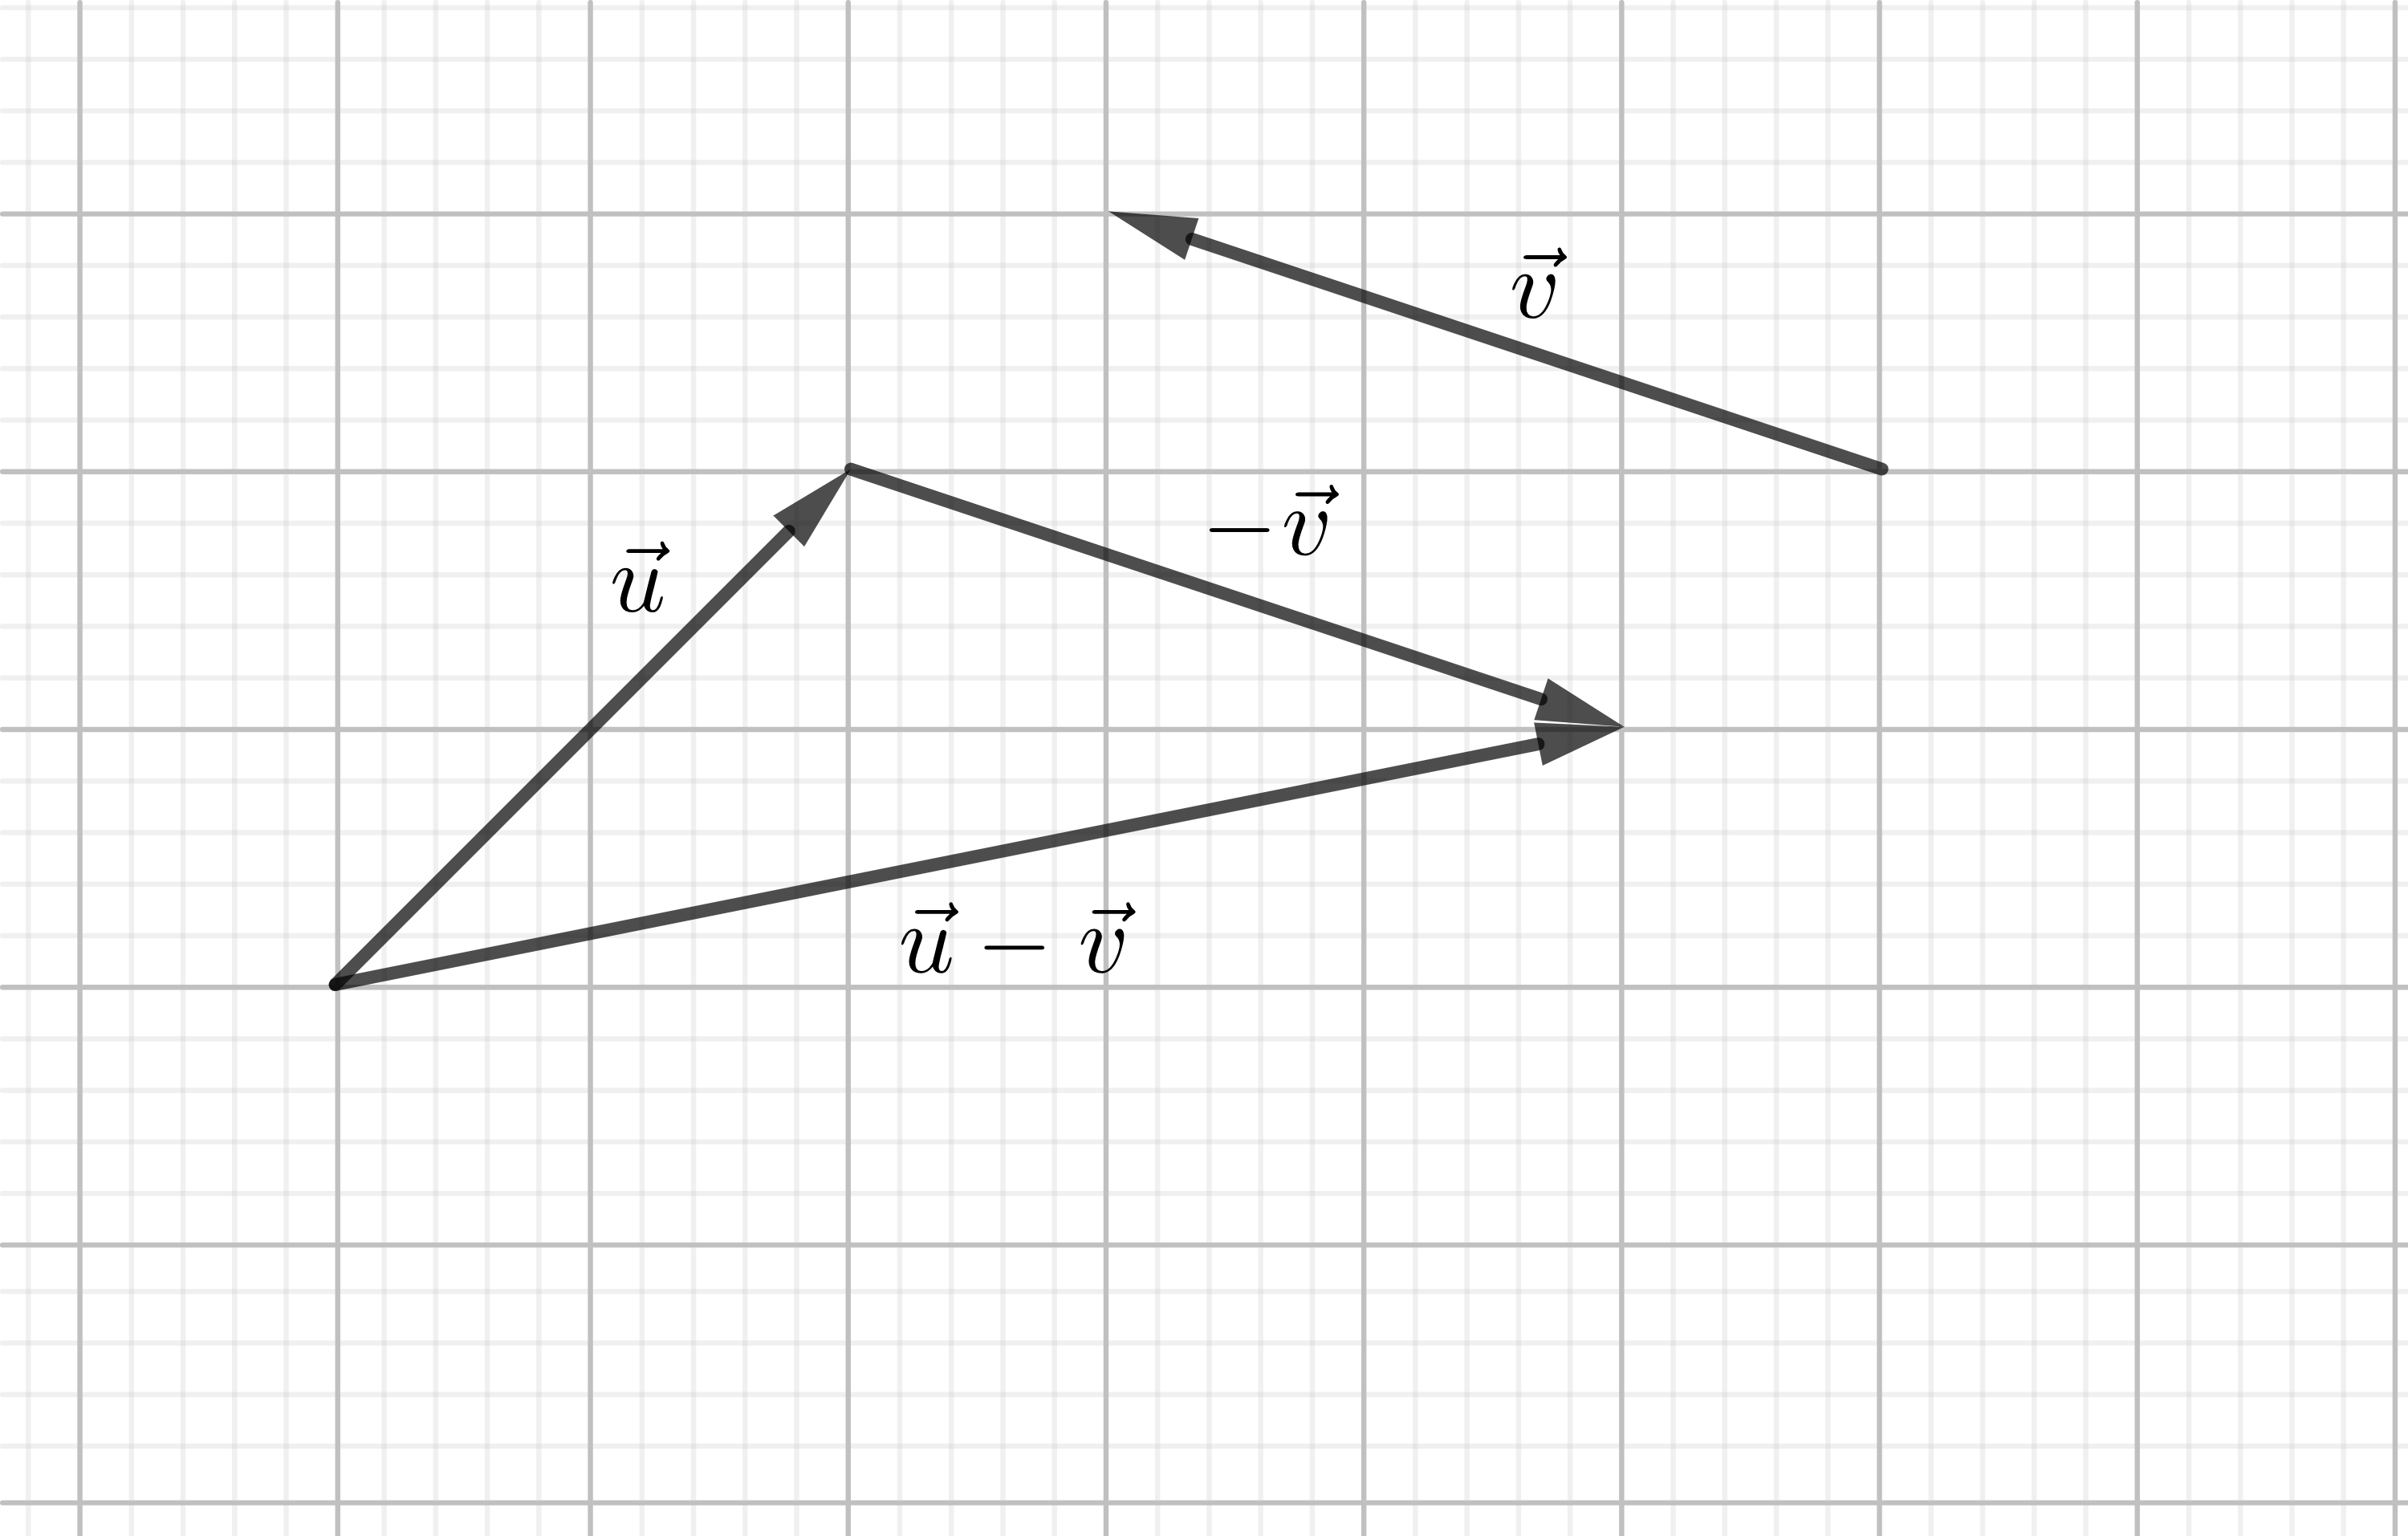
\includegraphics[width=0.7\textwidth]{./cap_vetor/dados/fig_vsubtracao/fig_vsubtracao}
  \caption{Representação geométrica da subtração de $\vec{u}$ com $\vec{v}$, i.e. $\vec{u}-\vec{v}$.}
  \label{fig:vsubtracao}
\end{figure}

\begin{obs}\normalfont{(Regra do paralelograma)}
  Sejam vetores não nulos $\vec{u} = \overrightarrow{AB}$ e $\vec{v} = \overrightarrow{AC}$. Seja, ainda, $D$ o vértice oposto a $A$ no paralelograma determinado pelos lados formados pelos segmentos $AB$ e $AC$. Então, temos $\vec{u} + \vec{v} = \overrightarrow{AD}$ e $\vec{u}-\vec{v} = \overrightarrow{CD}$. Veja a Figura \ref{fig:regrapara}.

\begin{figure}[H]
  \centering
  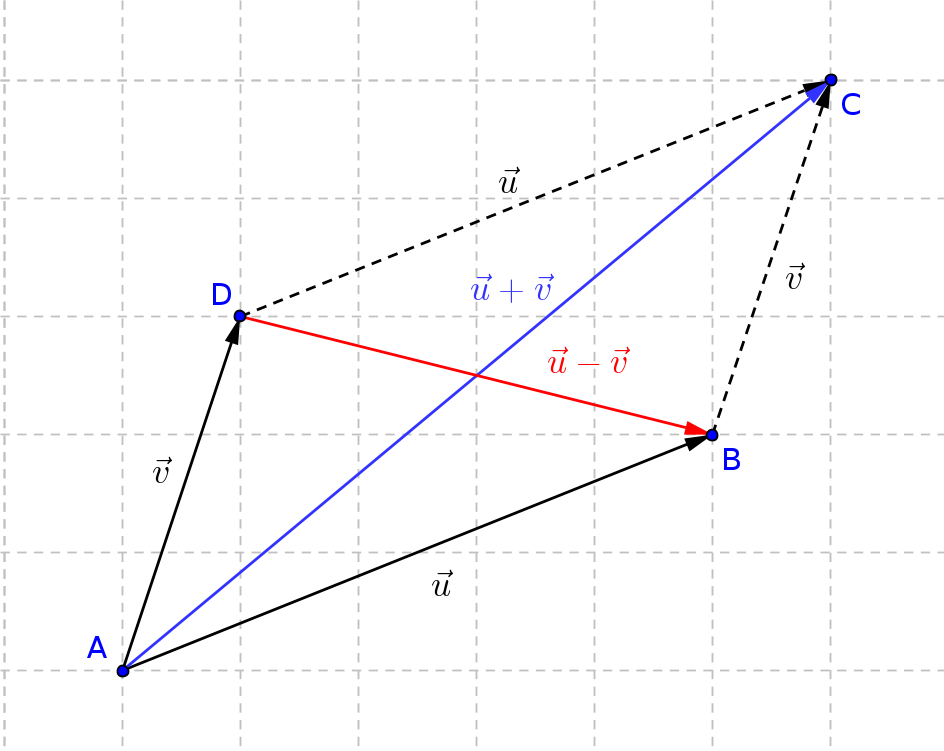
\includegraphics[width=0.7\textwidth]{./cap_vetor/dados/fig_regrapara/fig_regrapara}
  \caption{Regra do paralelograma para a presentação geométrica da soma e da diferença de vetores.}
  \label{fig:regrapara}
\end{figure}  
\end{obs}

\subsection{Multiplicação de vetor por um escalar}

A multiplicação de um número real $\alpha>0$ (escalar) por um vetor $\vec{u}$ é denotado por $\alpha\vec{u}$ e é definido pelo vetor de mesma direção e mesmo sentido de $\vec{u}$ com norma $\alpha|\vec{u}|$. Quando $\alpha = 0$, define-se $\alpha\vec{u}=\vec{0}$, i.e. o vetor nulo (geometricamente, representado por qualquer ponto).

\begin{obs}
  \begin{itemize}
  \item Para $\alpha<0$, temos $\alpha\vec{u} = -(-\alpha\vec{u})$.
  \item $|\alpha\vec{u}|=|\alpha||\vec{u}|$.
\end{itemize}
\end{obs}

\begin{figure}[h!]
  \centering
  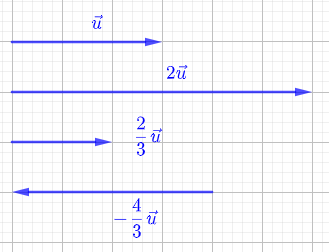
\includegraphics[width=0.7\textwidth]{./cap_vetor/dados/fig_vescalar/fig_vescalar}
  \caption{Representações geométricas de multiplicações de um vetor por diferentes escalares.}
  \label{fig:vescalar}
\end{figure}

\begin{obs}
  As seguintes propriedades são válidas:
  \begin{enumerate}[a)]
  \item Associatividade da multiplicação por escalar:
    \begin{equation}
      \alpha\left(\beta\vec{u}\right) = (\alpha\beta)\vec{u}
    \end{equation}

    De fato, em primeiro lugar, observamos que $\alpha\left(\beta\vec{u}\right)$ e $(\alpha\beta)\vec{u}$ têm a mesma direção e o mesmo sentido. Por fim, temos
    \begin{align}
      |\alpha\left(\beta\vec{u}\right)| &= |\alpha||\beta\vec{u}| \\
                                        &= |\alpha|\left(|\beta||\vec{u}|\right) \\
                                        &= \left(|\alpha||\beta|\right)|\vec{u}| \\
                                        &= |\alpha\beta||\vec{u}| \\
                                        &= |(\alpha\beta)\vec{u}|.
    \end{align}
    
  \item Distributividade:
    \begin{align}
      &(\alpha + \beta)\vec{u} = \alpha\vec{u} + \beta\vec{u}\\
      &\alpha\left(\vec{u}+\vec{v}\right) = \alpha\vec{u} + \alpha\vec{v}
    \end{align}
  \end{enumerate}
\end{obs}

\subsection{Resumo das propriedades das operações com vetores}

As operações de adição e multiplicação por escalar de vetores têm propriedades importantes. Para quaisquer vetores $\vec{u}$, $\vec{v}$ e $\vec{w}$ e quaisquer escalares $\alpha$ e $\beta$ temos:
\begin{itemize}
\item comutatividade da adição: $\vec{u}+\vec{v}=\vec{v}+\vec{u}$;
\item associatividade da adição: $(\vec{u} + \vec{v}) + \vec{w} = \vec{u} + (\vec{v} + \vec{w})$;
\item elemento neutro da adição: $\vec{u}+\vec{0}=\vec{u}$;
\item existência do oposto: $\vec{u}+(-\vec{u}) = \vec{0}$;
\item associatividade da multiplicação por escalar: $\alpha(\beta\vec{u})=(\alpha\beta)\vec{u}$;
\item distributividade da multiplicação por escalar:
  \begin{align}
    &\alpha(\vec{u}+\vec{v}) = \alpha\vec{u}+\alpha\vec{v},\\
    &(\alpha+\beta)\vec{u} = \alpha\vec{u}+\beta\vec{u};
  \end{align}
\item existência do elemento neutro da multiplicação por escalar: $1\vec{u}=\vec{u}$.
\end{itemize}

\subsection*{Exercícios resolvidos}

\begin{exeresol}
  Mostre que $\vec{u} + \vec{v} = \vec{v} + \vec{u}$.
\end{exeresol}
\begin{resol}
  Seja $ABCD$ o paralelograma com $\vec{u} = \overrightarrow{AB} = \overrightarrow{DC}$ e $\vec{v} = \overrightarrow{AD} = \overrightarrow{BC}$. Logo, pela regra do paralelograma temos
  \begin{align}
    \vec{u} + \vec{v} &= \overrightarrow{AB} + \overrightarrow{BC} \\
                      &= \overrightarrow{AC} \\
                      &= \overrightarrow{AD} + \overrightarrow{DC} \\
                      &= \vec{v} + \vec{u}.
  \end{align}
\end{resol}

\subsection*{Exercícios}

\begin{exer}\label{exer:vetor_prob_01}
  Na figura abaixo, temos $\vec{u} = \overrightarrow{GJ}$ e $\vec{v} = \overrightarrow{AK}$. Assim sendo, escreva os vetores $\overrightarrow{RS}$, $\overrightarrow{NI}$, $\overrightarrow{AG}$, $\overrightarrow{NQ}$, $\overrightarrow{AT}$ e $\overrightarrow{PE}$ em função de $\vec{u}$ e $\vec{v}$.

  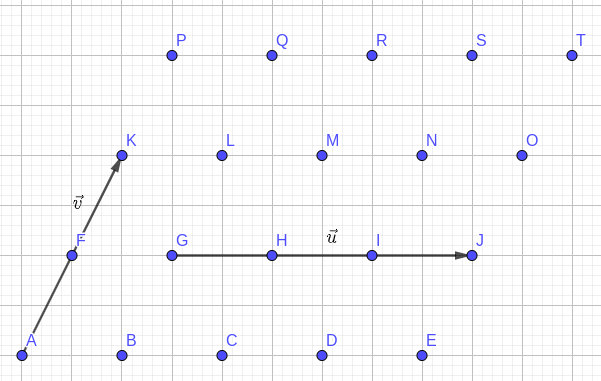
\includegraphics[width=0.7\textwidth]{./cap_vetor/dados/fig_exer_prob_01/fig_exer_prob_01}
\end{exer}

\begin{exer}\label{exer:vetor_prob_02}
  Sejam $\overrightarrow{CA}$, $\overrightarrow{CM}$ e $\overrightarrow{CB}$ os vetores indicados na figura abaixo. Mostre que $\overrightarrow{CM} = \frac{1}{2}\overrightarrow{CA} + \frac{1}{2}\overrightarrow{CB}$.

  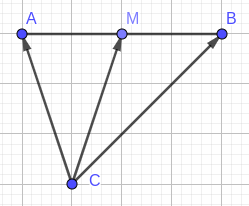
\includegraphics[width=0.7\textwidth]{./cap_vetor/dados/fig_exer_prob_02/fig_exer_prob_02}
\end{exer}
\begin{resp}
  Dica: $M$ é o ponto médio do segmento orientado $AB = CB - AC$.
\end{resp}

\begin{exer}
  Seja dado um vetor $\vec{u}\neq 0$. Calcule a norma do vetor $\vec{v}=\vec{u}/|\vec{u}|$\footnote{$\vec{u}/|\vec{u}|$ é chamado de vetor $\vec{u}$ normalizado, ou a normalização do vetor $\vec{u}$.}.
\end{exer}
\begin{resp}
  $|\vec{v}|=1$.
\end{resp}

\begin{exer}
  Diga se é verdadeira ou falsa cada uma das seguintes afirmações. Justifique sua resposta.
  \begin{enumerate}
  \item $\vec{u}+\vec{u} = 2\vec{u}$
  \item $\vec{u}=-\vec{u} \Leftrightarrow \vec{u} = \vec{0}$.
  \end{enumerate}
\end{exer}
\begin{resp}
  a) verdadeira; b) verdadeira.
\end{resp}
